\documentclass[12pt]{article}
\usepackage[dvips]{epsfig}
\usepackage{color}
\usepackage{url}
\usepackage[colorlinks=true]{hyperref}

\begin{document}

\section*{GENESIS: Documentation}

\section*{The GENESIS Graphic User Interface}

\section*{Introduction}

The GENESIS graphic user interface (GUI) provides an interactive environment for the construction, modification, and simulation of computational models of subcellular mechanisms, neurons and neural circuits.

The GUI is developed according to the principles of the Computational Biology Initiative Federated Software Architecture which is described in the \href{../genesis-overview/genesis-overview.tex}{GENESIS Overview}. The underlying philosophy of the GUI's modular software design is that it follows the \href{../work-flow/work-flow.tex}{GENESIS work flow} and supports the work flow's four basic steps:
\begin{enumerate}
\item {\bf Create/import, explore, and save model.}
\item {\bf Define simulation constants, inputs, and outputs.}
\item {\bf Check, run, reset simulation, and save model state.}
\item {\bf Check simulation output.}
\end{enumerate}
The block diagram given below illustrates the relationships between the software components that support this GUI functionality.

\begin{figure}[h]
  \centering
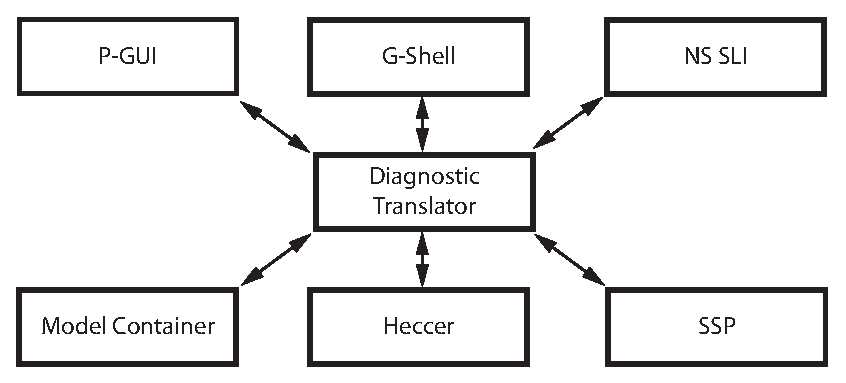
\includegraphics[scale=0.6]{figures/gui-isolated.eps}
%\caption{{\bf GUI software layout:} The GENESIS GUI is illustrated in this software block diagram.}
  \label{fig:df-1}
\end{figure}

\subsection*{User Interface Functions:} The GENESIS GUI can be initiated from either a \href{../unix-linux/unix-linux.tex}{UNIX prompt} or the \href{../gshell/gshell.tex}{G-shell}. Alternatively, There is a GUI that provides backward compatibility with previous versions of GENESIS (Version 2.3 and earlier).

\begin{itemize}
   \item {\bf P-GUI:} This refers to the initiation of a Python/Perl enabled GUI from the command line of a terminal window.
   \item {\bf G-shell:} The same GUI can also be initiated from the G-shell.
   \item {\bf NSSLI:} This refers to the Neurospaces Script Language Interpreter that provides backward compatibility with the Script Language Interpreter of earlier versions of GENESIS.
\end{itemize}

The Diagnostic Translator is a middle ware software component that enables interaction between the user (via a given GUI component--P-GUI, G-Shell, or NSSLI) and the \href{../model-container/model-container.tex}{Model Container}, \href{../heccer/heccer.tex}{Heccer}, or \href{../ssp/ssp.tex}{SSP}.

\end{document}
